\documentclass{beamer}
% September 2014 
% Author: Dr Rachid Hourizi and Dr. Michael Wright and Dr Michael Wright
% Department of Computer Science, University of Bath
\usepackage{listings}
\usetheme{Boadilla} 
\lstset{language=java,
	basicstyle=\ttfamily\small,
           keywordstyle=\color{blue}\ttfamily,
           stringstyle=\color{red}\ttfamily,
           commentstyle=\color{green}\ttfamily,
          breaklines=true}

\begin{document}

\AtBeginSection[]{
  \begin{frame}
  \vfill
  \centering
  \begin{beamercolorbox}[sep=8pt,center,shadow=true,rounded=true]{title}
    \usebeamerfont{title}\insertsectionhead\par%
  \end{beamercolorbox}
  \vfill
  \end{frame}
}

\title{CM 10227: Lecture 11}
\author{Dr. Rachid Hourizi and Dr. Michael Wright}
\date{\today}
\frame{\titlepage}

\begin{frame} 
\begin{center}
\textbf{Resources}
\end{center}
\begin{itemize}
\item More help with this course
\begin{itemize}
\item Moodle
\item E-mail - programming1@lists.bath.ac.uk
\end{itemize}
\item Online C and Java IDE
\begin{itemize}
\item https://www.codechef.com/ide
\item Remember to select Java from the drop down menu.
\end{itemize}
\item Books
\begin{itemize}
\item Java by Dissection (Free pdf online)
\item The Java Tutorial (https://docs.oracle.com/javase/tutorial/)
\end{itemize}
\end{itemize}
\end{frame}

\begin{frame} 
\begin{center}
\textbf{Resources}
\end{center}
\begin{itemize}
\item The places that you can get additional support if you are finding the pace of the course a little fast now include
\begin{itemize}
\item A labs (Continued from week 1)
\item B labs 
\item ... Wednesday 11:15-13:05 EB0.7
\item ... Fridays 17:15 to 19:15 in CB 5.13)
\item The Drop in Session 
\item ... booked 20 min appointments
\item ... Friday 11.15-13.05 1E 3.9
\item PAL sessions (Mondays 14:15 to 15:05 1E 3.9)
\end{itemize}
\end{itemize}
\end{frame}

% *** Last week ***
\begin{frame}
\begin{center}
\textbf{Last Week}
\end{center}
\begin{itemize}
\item Java API Libraries
\end{itemize}
\end{frame}

% *** This week ***
\begin{frame}
\begin{center}
\textbf{This Week}
\end{center}
\begin{itemize}
\item Complexity
\end{itemize}
\end{frame}

% CONTENT 
\section{Complexity}
\begin{frame}
\begin{itemize}
\item To this point in the course, we have, on a number of occasions talked about algorithms, pseudo code and
implementation (more detailed definitions of each one will follow, below)
\item We have also discussed the fact that most if not all programming problems can be approached in many different ways
\item i.e. that different algorithms can be employed to address the challenges of a given programming task
\end{itemize}
\end{frame} 

\begin{frame}
\begin{itemize}
\item That different programmers will take different approaches to developing pseudo-code when fleshing out the details of a given algorithm ...
\item ... and that even quite detailed pseudo code leaves room for different programmers to make different design decisions
during implementation
\item We have not, yet, however talked about the ways in which we might compare algorithms (i.e. decide whether one is
`better' or another `worse')
\end{itemize}
\end{frame} 

\begin{frame}
\begin{definition}{Algorithm:}
a process or set of rules to be followed in calculations or other problem-solving operations
\end{definition}

\begin{definition}{Pseudo Code:}
a notation resembling a simplified programming language, used in program design.
\end{definition}

\begin{definition}{Implementation:}
the process of putting a decision or plan into effect; execution.
\end{definition}
\end{frame}

\begin{frame}
\begin{center}
\textbf{Problem...}
\end{center}
\begin{itemize}
\item We need a machine, implementation independent way of comparing algorithms
\end{itemize}
\end{frame} 

\begin{frame}
\begin{itemize}
\item Complexity is a (the?) way we can tell whether one method is better than another.
\item We get a measure of how long an algorithm will take to get the answer.
\item We seek a measure of the size of a problem: e.g., number of items to sort, numbers of items to search, but this can be any other measure we wish.
\end{itemize}
\end{frame} 

\begin{frame}
\begin{itemize}
\item We need to know
\begin{itemize}
\item how long it will take to solve, and
\item how much memory the solution will need.
\end{itemize}
\item It's good to have an estimate of these two; time complexity and space complexity.
\end{itemize}
\end{frame} 

\section{Big O notation}

\begin{frame}
\begin{itemize}
\item We need some basic vocabulary to describe the behaviours.
\item The basic idea is that we have the size of the problem (n), and we want to determine how long it takes to run/how much memory it takes/etc., and how that depends on n.
\end{itemize}
\end{frame} 

\begin{frame}
\begin{itemize}
\item 10n\textsuperscript{3} + 15n\textsuperscript{2} + 20 = 45 (where n = 1)
\bigskip
\item n = 2 : 10n\textsuperscript{3} + 15n\textsuperscript{2} + 20 = 160
\bigskip
\item n = 10 : 10n\textsuperscript{3} + 15n\textsuperscript{2} + 20 = 11,520
\bigskip
\item n = 10 : (10 x \textbf{\underline{1000}}) + (15 x 100) + 20 = 11,520
\bigskip
\item O(n\textsuperscript{3})
\end{itemize}
\end{frame} 

\begin{frame}[fragile]
Example : Constant Complexity - O(1)
\begin{block}{}
\begin{lstlisting}
private int[] myArray = new int[100000];
private int index = 0;

public void addItemToArray(int value){
    myArray[index] = value;
    index++;
}
\end{lstlisting}
\end{block}
\end{frame} 

\begin{frame}[fragile]
Example : Linear Complexity - O(n)
\begin{block}{}
\begin{lstlisting}
private int[] myArray = new int[100000];

public void fillMyArray(int value){
    for(int i=0; i<myArray.length; i++){
        myArray[i] = value;
    }
}
\end{lstlisting}
\end{block}
\end{frame} 

\begin{frame}[fragile]
Example : Quadratic Complexity - O(n\textsuperscript{2})
\begin{block}{}
\begin{lstlisting}
private int[] myArray = new int[100000];

public void fillMyArray(int value){
    for(int i=0; i<myArray.length; i++){
        int sum = i;
        for(int j=0; j<myArray.length; j++){
            sum += myArray[j];
        }
        myArray[i] = value+sum;
    }
}
\end{lstlisting}
\end{block}
\end{frame}

\begin{frame}[fragile]
Example : Logarithmic Complexity - O(log n)
\begin{block}{}
\begin{lstlisting}
public void printSomeValues(int value){
    for(int i=1; i<value; i=i*2){
        System.out.println(i + ", ");
    }
}

public void printSomeOtherValues(int value){
    for(int i=value; i>1; i=i/2){
        System.out.println(i + ", ");
    }
}
\end{lstlisting}
\end{block}
\end{frame}

\begin{frame}[fragile]
Example : Exponential Complexity - O(2\textsuperscript{n})
\begin{block}{}
\begin{lstlisting}
public int fib(int number){
    if (number <= 1){ 
        return number;
    }
    else{
        return fib(number - 2) + fib(number - 1);
    }
}
\end{lstlisting}
\end{block}
\end{frame}

\begin{frame}
\begin{itemize}
\item Suppose we find two algorithms that take times \textit{n}\textsuperscript{2 }and 100\textit{n }to run respectively.
\item At first, the \textit{n}\textsuperscript{2 }seems better, but the square term is eventually going to dominate:
\item For n= 1million, n squared is a quadrillion. So the 100\textit{n }algorithm is actually the better one (for large
datasets).
\end{itemize}
\end{frame} 

\begin{frame}
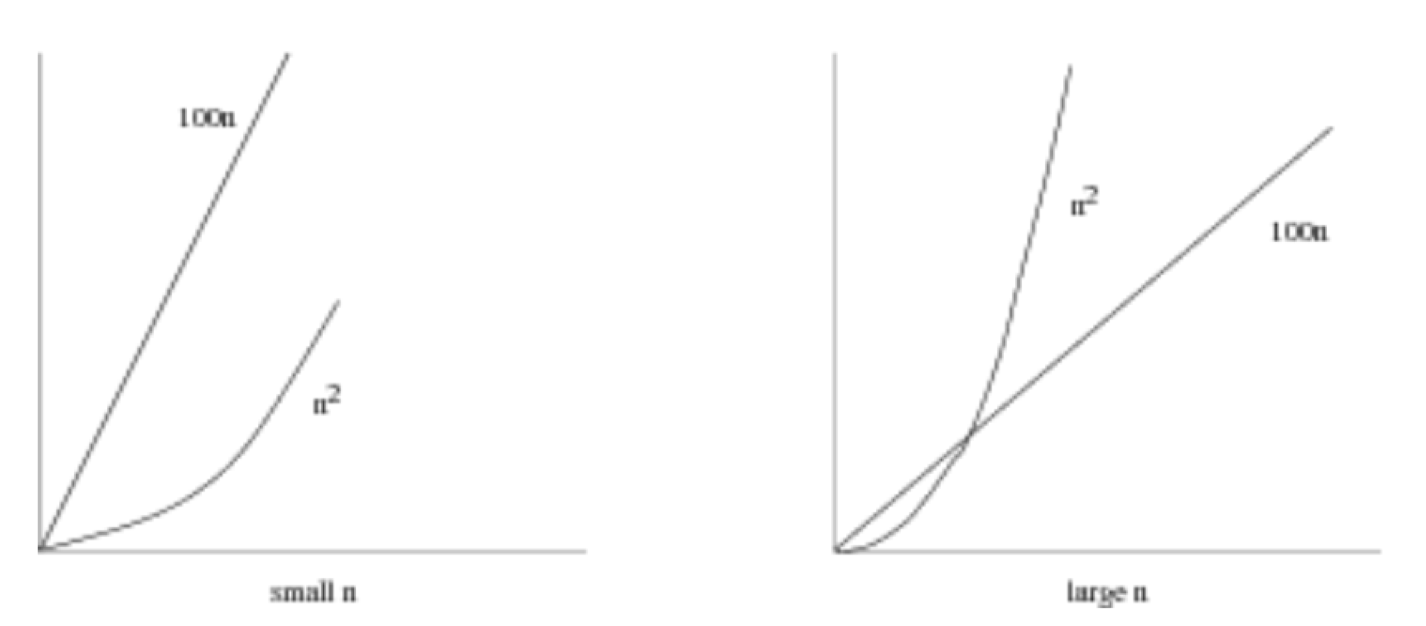
\includegraphics[height=5cm,keepaspectratio]{images/image1}
\end{frame} 

\begin{frame}
\begin{itemize}
\item Next, suppose we have an algorithm that takes time \textit{n}\textsuperscript{2 }+ 100\textit{n}.
\item For \textit{n }= 1000000, the 100\textit{n }is 100 million, which is just 1/100\% of a quadrillion.
\item So when we are talking about big values for \textit{n }we need only think about the quadratic term as that forms
the overwhelming part of the time.
\item The linear term is important for small \textit{n}, but we are really concerned with big \textit{n}.
\item We can simplify by ignoring the small stuff.
\end{itemize}
\end{frame} 

\begin{frame}
\begin{itemize}
\item We say the problem has complexity \textit{O}(\textit{n}\textsuperscript{2}). 
\item This notation means that the problem grows like \textit{an}\textsuperscript{2 }+ stuff where \textit{a }is some constant, and ``stuff''
grows slower than \textit{n}\textsuperscript{2}, and so will be minuscule relative to \textit{n}\textsuperscript{2 }for
large \textit{n}
\item this statement is valid for all large enough values of \textit{n }
\item this statement says nothing about small \textit{n}, or what ``large enough'' is supposed to mean
\item we're not too concerned as to whether it is 100\textit{n}\textsuperscript{2 }+ stuff or
2\textit{n}\textsuperscript{2 }+ stuff
\end{itemize}
\end{frame} 

\begin{frame}
\begin{itemize}
\item The important part is how the time grows with \textit{n}.
\item All sorts of factors determine the actual time a program takes to run: the speed of the computer, how good the
compiler of the language is, whether the processor has a good multiply operation, and so on.
\item It is much more useful to compare relative times for various sizes of problem, i.e., \textit{n}.
\item If the complexity is \textit{O}(2\textit{\textsuperscript{n}}), if a problem of size \textit{n }= 10 is doubled it takes 2\textsuperscript{10 }=1024 times as long. 
(because 2\textsuperscript{2}\textit{\textsuperscript{n}}/2\textit{\textsuperscript{n }}=2\textit{\textsuperscript{n}})  
\item If a problem of size \textit{n }= 100 is doubled it takes 2\textsuperscript{100 }or approx.. 10\textsuperscript{30
}times as long.
\end{itemize}
\end{frame} 

\begin{frame}
\begin{itemize}
\item It's best to avoid solutions that take exponential time, but some problems don't appear to have faster solutions.
\item For example the \textbf{Travelling Salesman} (Given a list of cities and the distances between each pair of cities, what is the shortest possible route that visits each city exactly once and returns to the origin city?)
\item Note that just because they don't \textit{appear }to have fast solutions doesn't mean they don't!
\item New solutions to old problems are being found all the time.
\bigskip
\item The smaller the degree the better
\item Linear is nice, 
\item Logarithmic is better.
\end{itemize}
\end{frame} 

\begin{frame}
\begin{itemize}
\item There is a hierarchy:
\item constant {\textless} logarithmic {\textless} 1/\textit{r}th power {\textless} linear {\textless} quadratic
{\textless} \textit{r}th power {\textless} exponential
\end{itemize}

\begin{center}
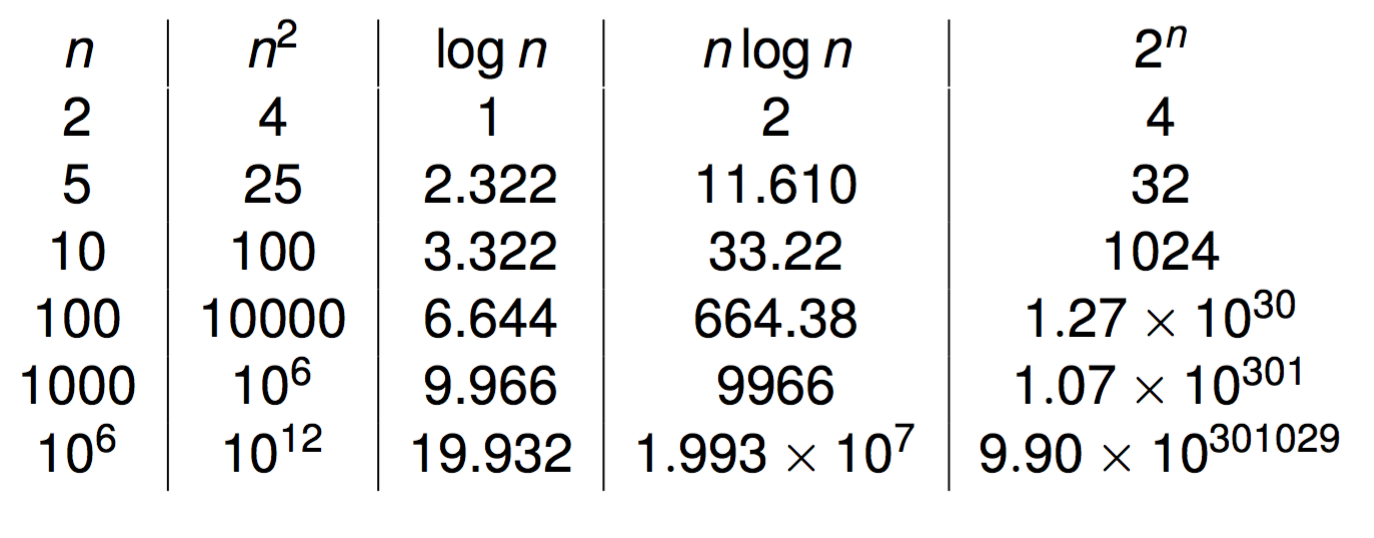
\includegraphics[height=4cm,keepaspectratio]{images/image2}
\end{center}

\end{frame} \begin{frame}

\begin{center}
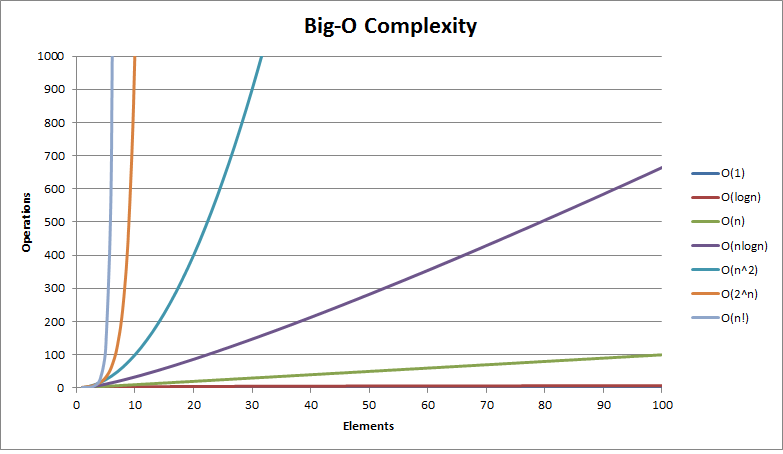
\includegraphics[height=7cm,keepaspectratio]{images/image3}
\end{center}

\end{frame} 

\section{Problems with Different Components}
\begin{frame}
\begin{itemize}
\item Suppose a problem that has two parts, the first takes time O(n), the second O(n2).
\item Taken together, the whole problem has complexity
\item O(n) + O(n\textsuperscript{2}) = O(n\textsuperscript{2}), as the linear part can be disregarded for large n.
\item Note this does not imply that O(n) = 0 
\item It means that c\textsubscript{1}n + c\textsubscript{2}n\textsuperscript{2} {\textless} cn\textsuperscript{2} for some c and large n.
\item Similarly, if a problem has two parts, both taking time O(n), then the total is O(n) + O(n) = O(n).
\item A problem of complexity O(1) is one that takes no more than a constant time to solve, regardless of its size.
Again, that the constant time could be 1ms or 1 million years: the important point is it is independent of n. 
\item Here the hidden constant can be very important.
\end{itemize}
\end{frame} 

\begin{frame}
\begin{itemize}
\item Slow functions...
\bigskip
\item Confusingly, we say a function is slow if it grows slowly (like log).
\item When an algorithm complexity corresponds to a slow function, it is fast, i.e., the time it takes to run increases
slowly.
\end{itemize} 
\end{frame} 

\begin{frame}
\begin{itemize}
\item Cases - Algorithms are measured in many ways, but some popular cases are
\bigskip
\item Best case: What is the best possible situation for this algorithm? Data are allowed to be in just the right values
and in just the right places to make the algorithm perform at its best.
\item Average case: What happens in the average case? This should be the behaviour we would expect to see normally with
data that are in no particular configuration.
\end{itemize}
\end{frame} 

\begin{frame} 
\begin{itemize}
\item Worst case: What is the worst that can happen? When the data happen to be in just the wrong configuration.
\item Common case: Is there something special we know about the data we can use to our advantage? For example, nearly
sorted data. Ideally, we want the common case to be the same as the best case.
\end{itemize}
\end{frame} 

\section{Sorting Algorithms and their Complexity}
\begin{frame}
\begin{itemize}
\item Lets look at some example of sorting and think about their complexity
\bigskip
\item Selection Sort
\item Insertion Sort 
\item Bubble Sort 
\item Merge Sort 
\item Quick Sort
\end{itemize}

\end{frame} 

\section{Selection Sort}
\begin{frame}[fragile]

Selection sort pseudocode

\begin{block}{}
\begin{lstlisting}
function selection_sort(int[] A):
// given a list A of n numbers indexed 0 to n-1
    for i from 0 to n-2
        k=i //index of the smallest value so far
        for j from i+ to n-1
            if A[j] < A[k]
            then k=j
        swap A[i] and A[k]
\end{lstlisting}
\end{block}
\end{frame} 

\begin{frame}
\begin{center}
\textbf{Selection Sort Complexity}
\end{center}
\begin{itemize}
\item The complexity of this algorithm is fairly easy to compute:
\item the first \textit{i} loop takes \textit{n}steps, 
\item the next \textit{n }$-$ 1, and so on. 
\bigskip
\item The total is 
\item \textit{n}+(\textit{n}$-$1)+(\textit{n}$-$2)+{\textperiodcentered}{\textperiodcentered}{\textperiodcentered}+3+2=
\textit{n}(\textit{n }+ 1)/2 $-$ 1 = \textit{O}(\textit{n}\textsuperscript{2})
\item Notice this time is independent of the data: even if the data
\item is already sorted it takes \textit{O}(\textit{n}\textsuperscript{2}) time!
\end{itemize}

\end{frame} 

\begin{frame}
\begin{center}
\textbf{Selection Sort Complexity}
\end{center}
\begin{itemize}
\item Time: best O(n\textsuperscript{2}), average O(n\textsuperscript{2}), worst O(n\textsuperscript{2}).
\item Space O(n). More precisely: n + O(1)
\item Other criteria: moves items directly to their destination, which can be important if the cost of moving is high. 
\item A quadratic algorithm, so bad for large datasets.
\end{itemize}

\end{frame} 

\begin{frame}
\begin{center}
\textbf{Finer Comparisons}
\end{center}
\begin{itemize}
\item Sometimes the complexity of sorting algorithms is more finely subdivided.
\item We might not just count the number of steps, but also

\begin{itemize}
\item the number of comparisons made, 
\item and the number of moves made.
\end{itemize}
\item For example, selection sort takes O(n\textsuperscript{2}) comparisons but only O(n) moves.
\end{itemize}

\end{frame} 

\begin{frame}
\begin{itemize}
\item Sometimes moving an object is much more expensive than comparing
\item Example: think of sorting a line of cars into number plate order: 
\item (you want to move the cars as little as possible).
\item In such a case you might want an algorithm that uses as few moves as possible, even to the extent of doing a lot
more comparisons.
\item Sometimes, a comparison is more expensive than a move. 
\item In this case you would want to minimise comparisons.
\item For example, when sorting long strings of nearly-identical DNA into order, the comparison would be quite costly.
\end{itemize}
\end{frame} 

\section{Insert Sort}
\begin{frame}[fragile]

Insert Sort: Algorithm

\begin{block}{}
\begin{lstlisting}
function insertion_sort(int[] A): 
    for i = 1 to length(A) - 1
        j = i
        while j > 0 and A[j-1] > A[j]
            swap A[j] and A[j-1]
            j = j - 1
        end while
    end for

\end{lstlisting}
\end{block}

What is the worst case complexity?
\end{frame} 

\begin{frame}
\begin{center}
\textbf{Insert Sort Complexity}
\end{center}
\begin{itemize}
\item If the data are already ordered, the \textit{j }loop exits immediately every time, and we take
\textit{O}(\textit{n}) steps.
\item If not, the comparing against the sorted part takes
1+2+3+{\textperiodcentered}{\textperiodcentered}{\textperiodcentered}+(\textit{n}$-$2)=\textit{O}(\textit{n}\textsuperscript{2})
steps again.
\item Time: best O(n), average O(n\textsuperscript{2}), worst O(n\textsuperscript{2}). 
\item Space: O(n)
\item Other criteria: exceptionally good for nearly sorted data. Low overhead, so good for small datasets. Bad, since
the O(n\textsuperscript{2}) means this performs really poorly for large datasets. A lot of shuffling, thus is poor if moving objects is
costly.
\item Comparisons: O(n\textsuperscript{2}). Moves: O(n\textsuperscript{2}).
\end{itemize} 

\end{frame} 

\section{Bubble Sort}
\begin{frame}
\begin{center}
\textbf{Bubble Sort Algorithm}
\end{center}
Repeatedly steps through the list to be sorted, compares each pair of adjacent items and swaps them if they are in the wrong order. The pass through the list is repeated until no swaps are needed, which indicates that the list is sorted\newline\newline
What is the best case complexity for bubble sort?
\end{frame} 

\begin{frame}[fragile]
\begin{block}{}
\begin{lstlisting}
function bubble_sort(int[] A): 
    n = length(A)
    repeat 
        swapped = false
        for i = 1 to n-1 inclusive do
            /* if this pair is out of order */
            if A[i-1] > A[i] then
                /* swap them and remember something changed */
                swap( A[i-1], A[i] )
                swapped = true
            end if
        end for
    until not swapped

\end{lstlisting}
\end{block}
\end{frame}

\begin{frame}
\begin{center}
\textbf{Bubble Sort Complexity}
\end{center}
\begin{itemize}
\item If the data are already sorted, we make one pass through and stop immediately.
\item Otherwise, we do about
\item (n $-$ 2) + (n $-$ 3) + {\textperiodcentered} {\textperiodcentered} {\textperiodcentered} + 3 + 2 + 1 = O(n\textsuperscript{2})
steps.
\end{itemize}

\end{frame} 

\begin{frame}
\begin{itemize}
\item Time: best O(n), average O(n\textsuperscript{2}), worst O(n\textsuperscript{2})
\item Space O(n).
\item Other criteria: good for nearly sorted data. Low overhead, so good for small datasets. Bad, since the O(n\textsuperscript{2}) means
this performs really poorly for large datasets.
\item Not so good for sorting lists. Comparisons: O(n\textsuperscript{2}). Moves: O(n\textsuperscript{2}).
\end{itemize}

\end{frame} 

\section{Merge Sort}
\begin{frame}[fragile]

Merge Sort: algorithm

\begin{block}{}
\begin{lstlisting}
function merge_sort(int[] A): 
    if(A.length == 1){
        return A;
    }
    else{
        return merge(merge_sort(A[0..A.length/2]), merge_sort(A[A.length/2..A.length]);
    }

function merge(int[] left, int[] right):
    int[] result;
    while left AND right are not empty:
        if first(left) <= first(right) then
            append first(left) to result
            left = rest(left)
        else
            append first(right) to result
            right = rest(right)
\end{lstlisting}
\end{block}

\end{frame} 

\begin{frame} 
\begin{center}
\textbf{Merge Sort Complexity}
\end{center}
\begin{itemize}
\item The complexity of this algorithm takes a little thought. 
\item The algorithm splits the list in half, sorts each half and then merges the two, so 
\item Time: best O(n log n), average O(n log n), worst O(n log n).
\item Space: 2n. 
\end{itemize}

\end{frame} 

\begin{frame}
\begin{itemize}
\item Other criteria: not so good as bubble sort with nearly sorted data.
\item Merge requires extra space or extra time to shuffle.Two list merge sort has very stable predictable
behaviour.
\item One improvement is not to recurse all the way down to single elements: better is to switch to, say, insertion sort
or even bubble sort when \textit{n }is small enough.
\item This takes advantage of the low overhead of such a sort and its speed on small datasets.
\end{itemize}

\end{frame} 

\section{Crossover of Bubble and Merge Sort}
\begin{frame}

\begin{center}
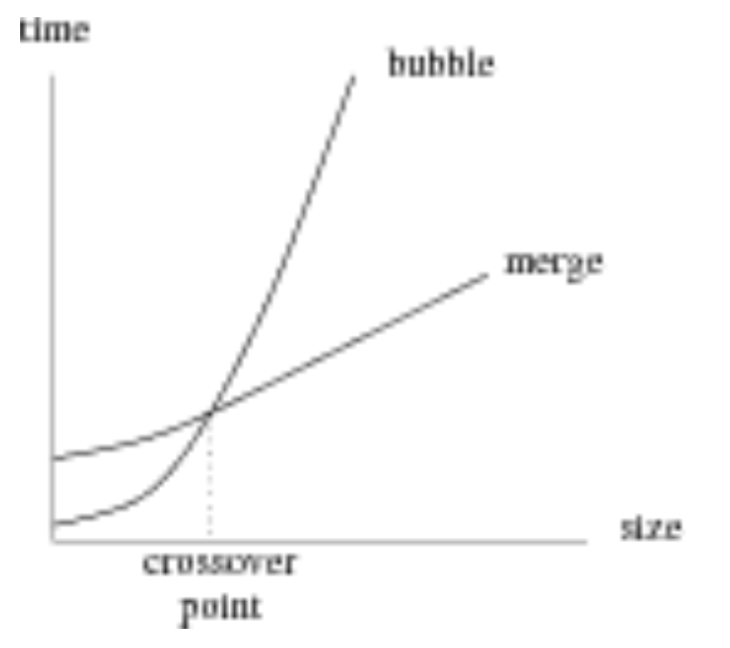
\includegraphics[height=7cm,keepaspectratio]{images/image4}
\end{center}

\end{frame} 

\begin{frame}
\begin{itemize}
\item The overhead of an algorithm is the amount of messing about in the algorithm that is needed to make it work but
doesn't really contribute much.
\item For example, shuffling in the mergesort is overhead bubblesort only has a tiny amount of overhead, but is a poor
algorithm.
\item mergesort has more overhead, but is a better algorithm.
\item This is why they have a crossover point: where the larger overhead is outweighed by the better algorithm.
\item The choice of algorithm is never easy to make!
\end{itemize}

\end{frame} 

\section{Quick Sort}
\begin{frame}

Quick Sort Algorithm

\begin{itemize}
\item Pick an element, called a pivot, from the array.
\item Partitioning: reorder the array so that all elements with values less than the pivot come before the pivot, while all elements with values greater than the pivot come after it (equal values can go either way). After this partitioning, the pivot is in its final position. This is called the partition operation.
\item Recursively apply the above steps to the sub-array of elements with smaller values and separately to the sub-array of elements with greater values.
\end{itemize}

\end{frame} 

\begin{frame}
\begin{center}
\textbf{Quick Sort Complexity}
\end{center}
\begin{itemize}
\item Just as with mergesort, we find the algorithm takes time O(n log n), if we get even splits every time.
\item Unfortunately, we can have bad splits too...
\item ... in the worst case we get a partition into 0 plus \textit{n }$-$ 1 elements
\item So, if we get bad splits, the time is \textit{O}(\textit{n}\textsuperscript{2}). 
\end{itemize}
\end{frame} 

\begin{frame}
\begin{itemize}
\item Choosing the pivot is critical
\item When the data is already sorted or nearly sorted, quicksort does really poorly.
\item Ditto for reversed or nearly reversed data.
\item It is a strange feature of quicksort that sorted data is its worst case!
\end{itemize}

\end{frame} 

\begin{frame} 
\begin{itemize}
\item Finding the pivot point
\bigskip
\item One approach, rather counter-intuitively, is to randomise the order of the data before using quicksort: this might
well give us a better run time!
\item Random element as pivot
\item Use two pivots
\item Use information about the pivots
\end{itemize}

\end{frame} 

\begin{frame}
\begin{itemize}
\item Quick sort finding the middle
\bigskip
\item It turns out that we can find the middle value of an array in O(n) time.
\item Consider the algorithm \textbf{select} which:
\bigskip
\item 1 consider the array in groups of 5 values: sort each 5 (using bubble sort, perhaps) and find the middle value of
each
\item 2 call select recursively on these middle values to find the overall middle value
\end{itemize}
\end{frame} 

\begin{frame}
\begin{itemize}
\item Using select to find a pivot, we can guarantee that quick sort has a good behaviour, with additional O(n log n)
time (O(n) for log n sort steps) taken to find the pivot.
\item Thus, still a total time of O(n log n), but somewhat longer than previously.
\item Of course, it may or may not be worthwhile spending this amount of time finding the pivot when one of the methods
above might be just as good: it all depends on the data.
\end{itemize}

\end{frame} 

\section{Combining Quicksort with Insertion Sort}
\begin{frame}
\begin{itemize}
\item Just as with any other divide and conquer method, there is no need to recurse all the way down to single elements
in quicksort.
\item Better is to stop at 3 or 4 elements and sort these directly;
\item or revert to insertion (or bubble, selection or other low-overhead sort) when the list is short enough.
\item This cut-over length must be determined experimentally as it will vary from implementation to implementation.
\end{itemize}

\end{frame} 

\begin{frame}
\begin{center}
\textbf{Summary}
\end{center}
\begin{itemize}
\item Looked at complexity and Big O notation
\item Examined complexity through different sorting algorithms
\end{itemize}
\end{frame} 

\end{document}
